\documentclass{article}




\usepackage[utf8]{inputenc}
\usepackage[T1]{fontenc}
\usepackage{amsmath} 
\usepackage{array}
\usepackage{xcolor}
\usepackage{amssymb}
\usepackage{amsthm}
\usepackage{graphicx}
\usepackage{float}


\newcommand\redu[1]{\color{red}\underline{\color{black}#1} \color{black}}
\newcommand\blueu[1]{\color{blue}\underline{\color{black}#1}\color{black}}
\newcommand\doubleu[1]{\underline{\underline{#1}}}



\author{Simon Wicky (260589) \and Jeremy Mion (261178)}
\title{Rapport Benchmarking DHT}
\date{05.2018}

\begin{document}

\maketitle
\pagenumbering{arabic}

\section{Benchmarking : Implémentation et scénarios testés}

\subsection{Implémentation}
L'implémentation de ce benchmarking en C est très brève. Elle consiste juste à chronométrer les phases réseau, c'est à dire la requête put ainsi que sa réponse, et la requête get, ainsi que sa réponse. Les différents scénario sont ensuite executés par l'intermédiaire de script bash, détaillés ci-après.

\subsection{Scénarios testés}
Les différents scénarios ont été testés :
\subsubsection{Put, couple clé-valeur fixe, N = 10, W variable}
Nous avons simulé 100 fois l'action de mettre une valeur sur la Hashtable, avec N valant 10, et W variant entre 1 et 10.\\
Le script \textbf{\textit{./test\_put}} effectue une action put, avec W partant de 1 jusqu'a 10. Le résultat est écrit dans un fichier. \\
Le script \textbf{\textit{./test\_put\_csv}} se charge de lancer 100 fois \textbf{\textit{./test\_put}}, de collecter les résultats et de les fusionner dans un seul fichier au format csv, où chaque ligne correspond à une valeur de W. \\
Les résultats récoltés sont résumés dans la Figure \ref{figPut}. 
\begin{figure}
 	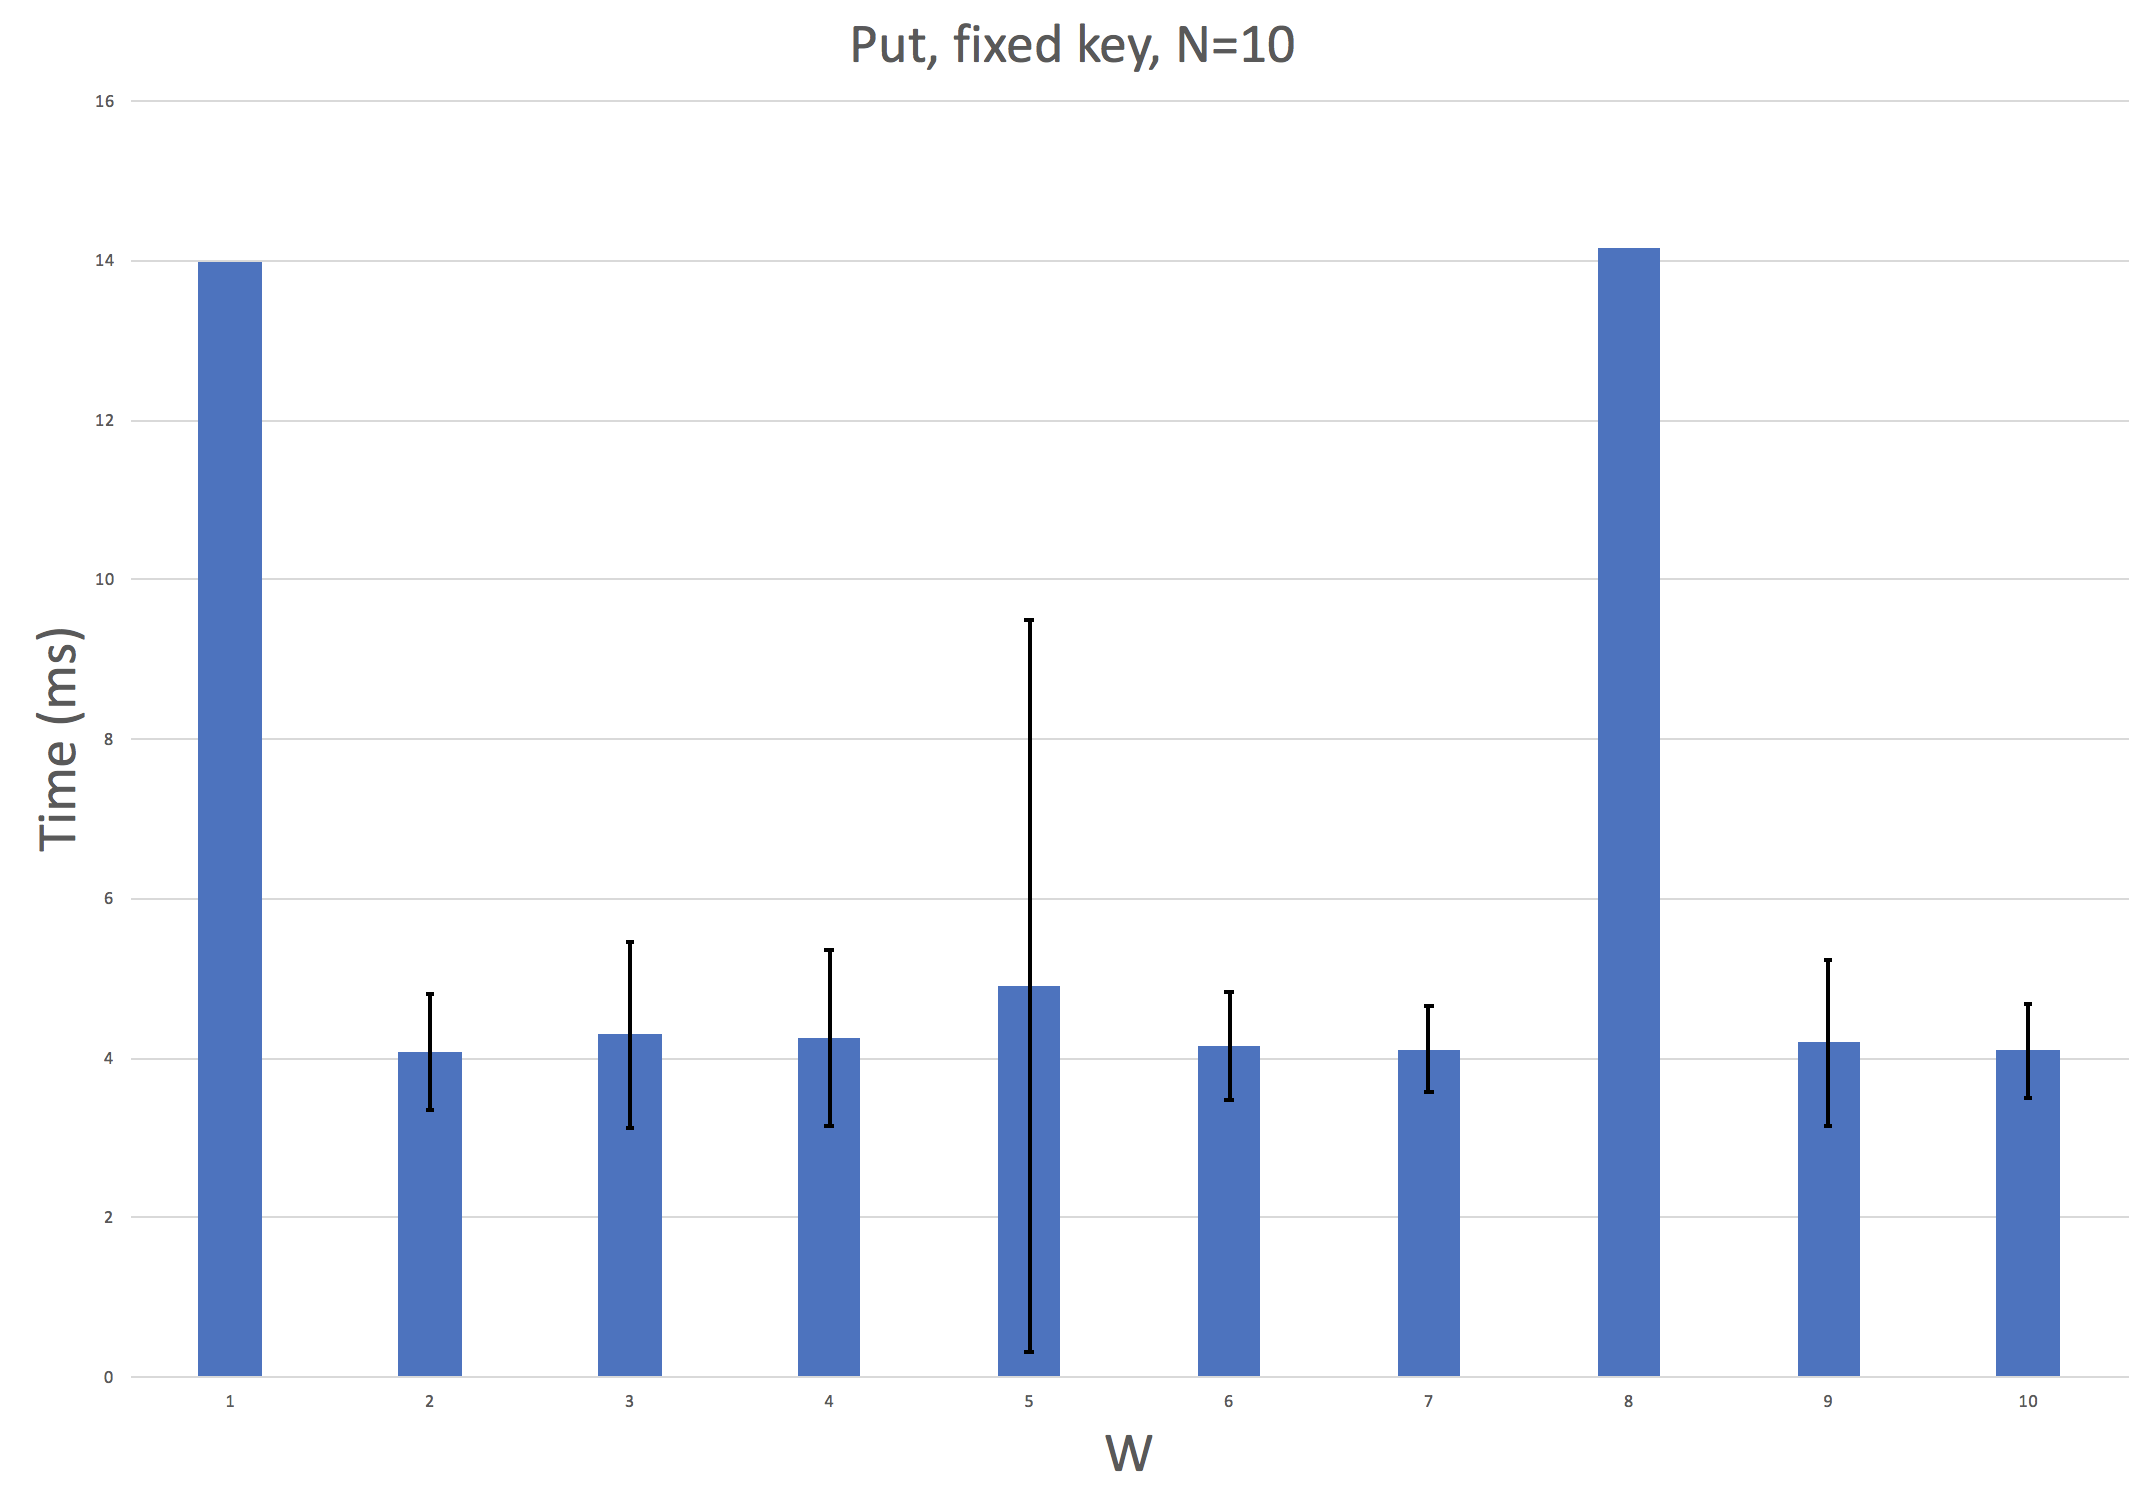
\includegraphics[scale = 0.25]{img/Put}
 	\caption{Graphique du scénarios 1.2.1}
 	\label{figPut}
\end{figure}

\subsubsection{Get, couple clé-valeur fixe, N = 10, R variable}
Nous avons ensuite simulé 100 fois l'action de demander une valeur sur la Hashtable, avec N valant 10, et R variant entre 1 et 10.\\
Le script \textbf{\textit{./test\_get}} effectue une action get, avec R partant de 1 jusqu'a 10. Le résultat est écrit dans un fichier. \\
Le script \textbf{\textit{./test\_get\_csv}} se charge de lancer 100 fois \textbf{\textit{./test\_get}}, de collecter les résultats et de les fusionner dans un seul fichier au format csv, où chaque ligne correspond à une valeur de R. \\
Les résultats récoltés sont résumés dans la Figure \ref{figGet}. 

\begin{figure}
 	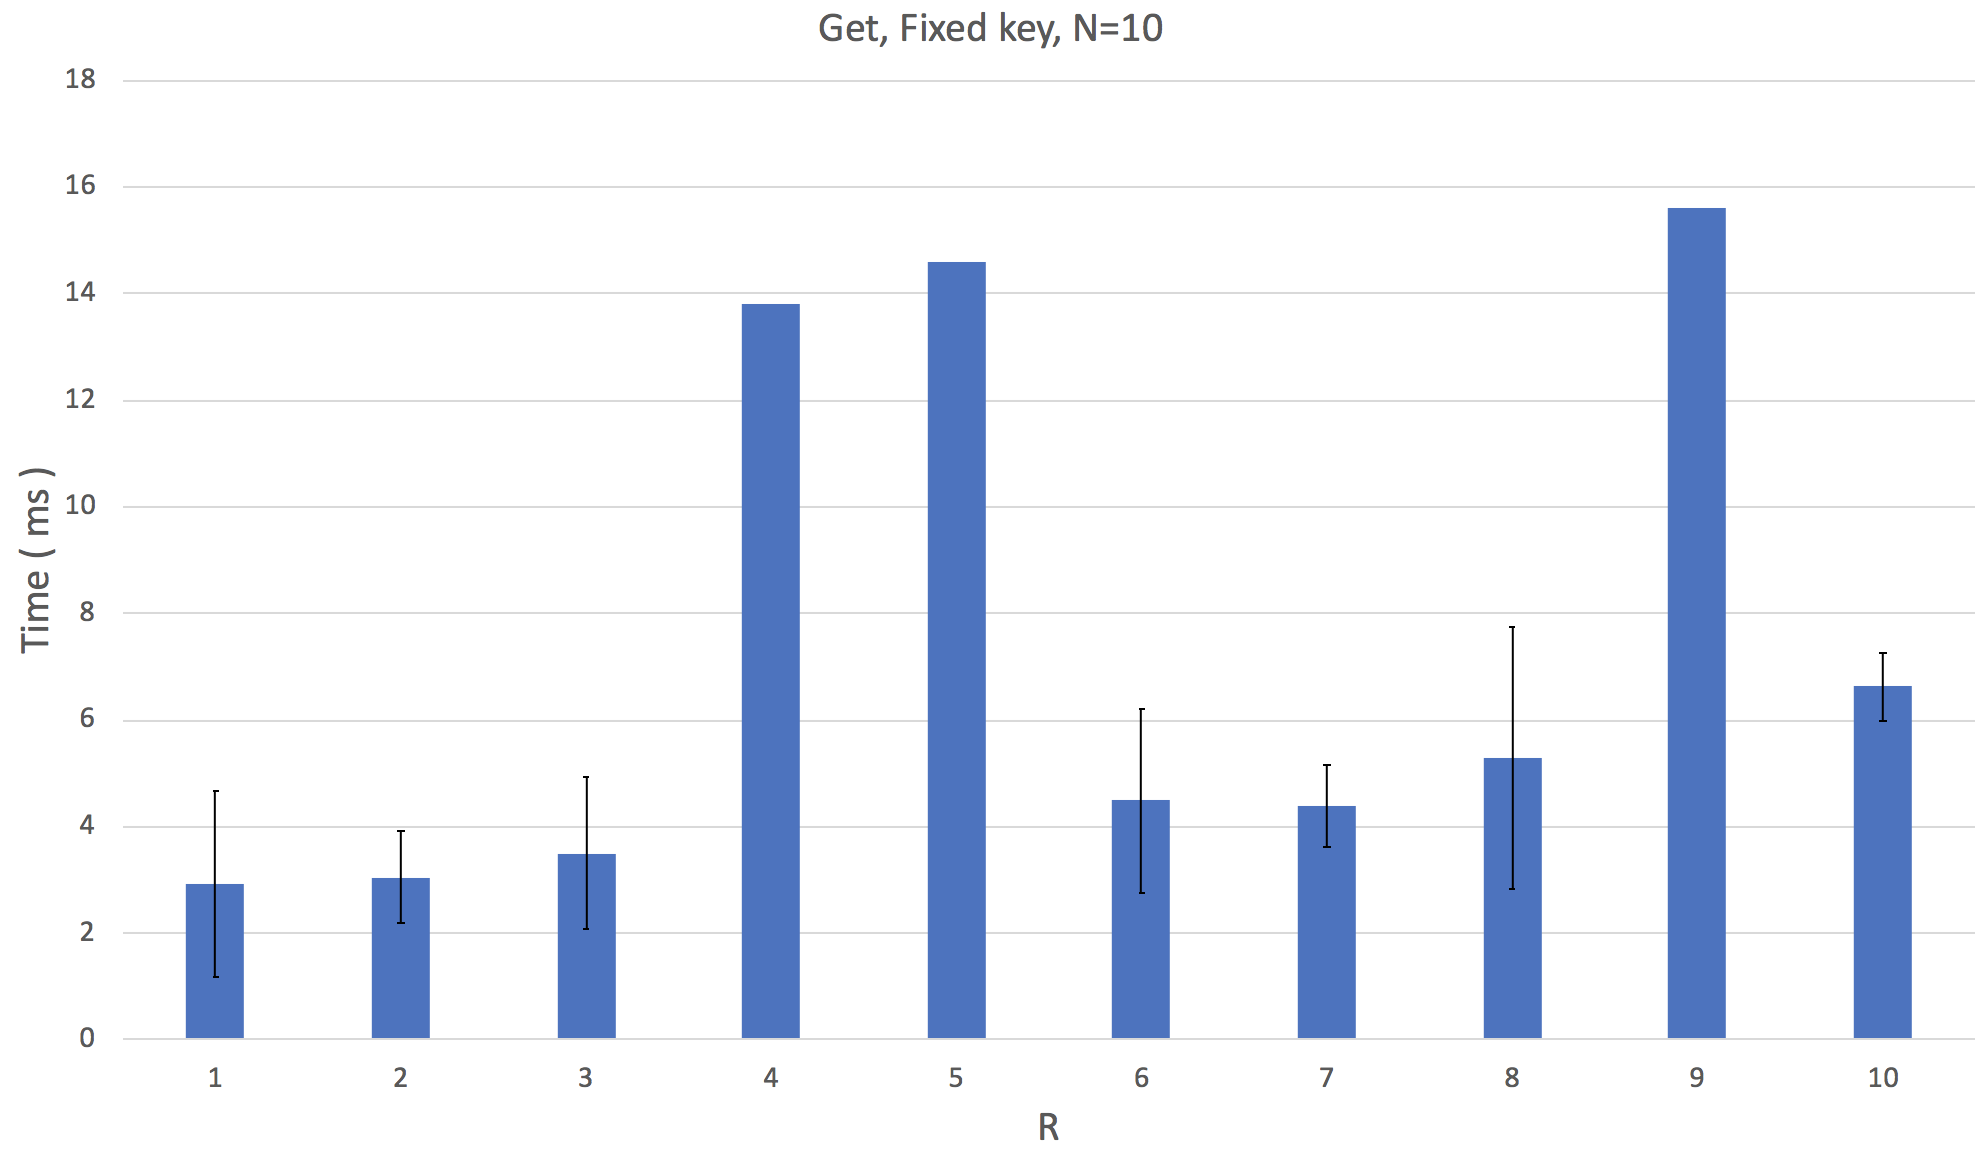
\includegraphics[scale = 0.25]{img/Get}
 	\caption{Graphique du scénarios 1.2.2}
 	\label{figGet}
\end{figure}





\end{document}
